\chapter{Конструкторская часть}

\section{Требования к разрабатываемому программному обеспечению}

К разрабатываемому статическому веб-серверу предъявляются следующие требования:
\begin{itemize}
	\item работа сервера в операционной системе на базе ядра Linux;
	\item соответствие сервера архитектуре prefork~+~pselect;
	\item поддержка запросов GET и HEAD;
	\item поддержка кодов состояний 200, 403, 404 и 405;
	\item поддержка HTML-, CSS-, JS-, PNG-, JPG-, JPEG-, SWF- и GIF-файлов;
	\item соответствие минимальным требованиям к безопасности статических серверов (ошибка в случае выхода адреса за корень директории сервера);
	\item обеспечение логирования.
\end{itemize}

\section{Сокеты}

Сокеты — название программного интерфейса для обеспечения обмена данными между процессами~\cite{socket}. Процессы при таком обмене могут исполняться как на одной электронной вычислительной машине, так и на различных компьютерах, связанных между собой сетью~\cite{socket}.

Каждый процесс может создать слушающий сокет и привязать его к определенному порту операционной системы~\cite{socket}.
Слушающий процесс обычно находится в цикле ожидания, то есть просыпается при появлении нового соединения~\cite{socket}.
При этом сохраняется возможность проверить наличие соединений на данный момент, установить тайм-аут для операции и так далее~\cite{socket}.

Каждый сокет имеет свой адрес~\cite{socket}.
ОС семейства UNIX могут поддерживать много типов адресов, но обязательными являются INET-адрес и UNIX-адрес~\cite{socket}.
Если привязать сокет к UNIX-адресу, то будет создан специальный файл по заданному пути, через который смогут общаться любые локальные процессы путем чтения или записи из него~\cite{socket}.
Сокеты типа INET доступны из сети и требуют выделения номера порта~\cite{socket}.
Обычно клиент явно подсоединяется к слушателю, после чего любое чтение или запись через его файловый дескриптор будут передавать данные между ним и сервером~\cite{socket}.
Все сокеты обычно ориентированы на применение датаграмм, но их точные характеристики зависят от интерфейса, обеспечиваемого протоколом~\cite{socket}.

На рисунке~\ref{linux_sock} представлен процесс установления соединения и обмена данными между сокетами сервера и клиента в операционной системе Linux.
\begin{figure}[H]
	\centering
	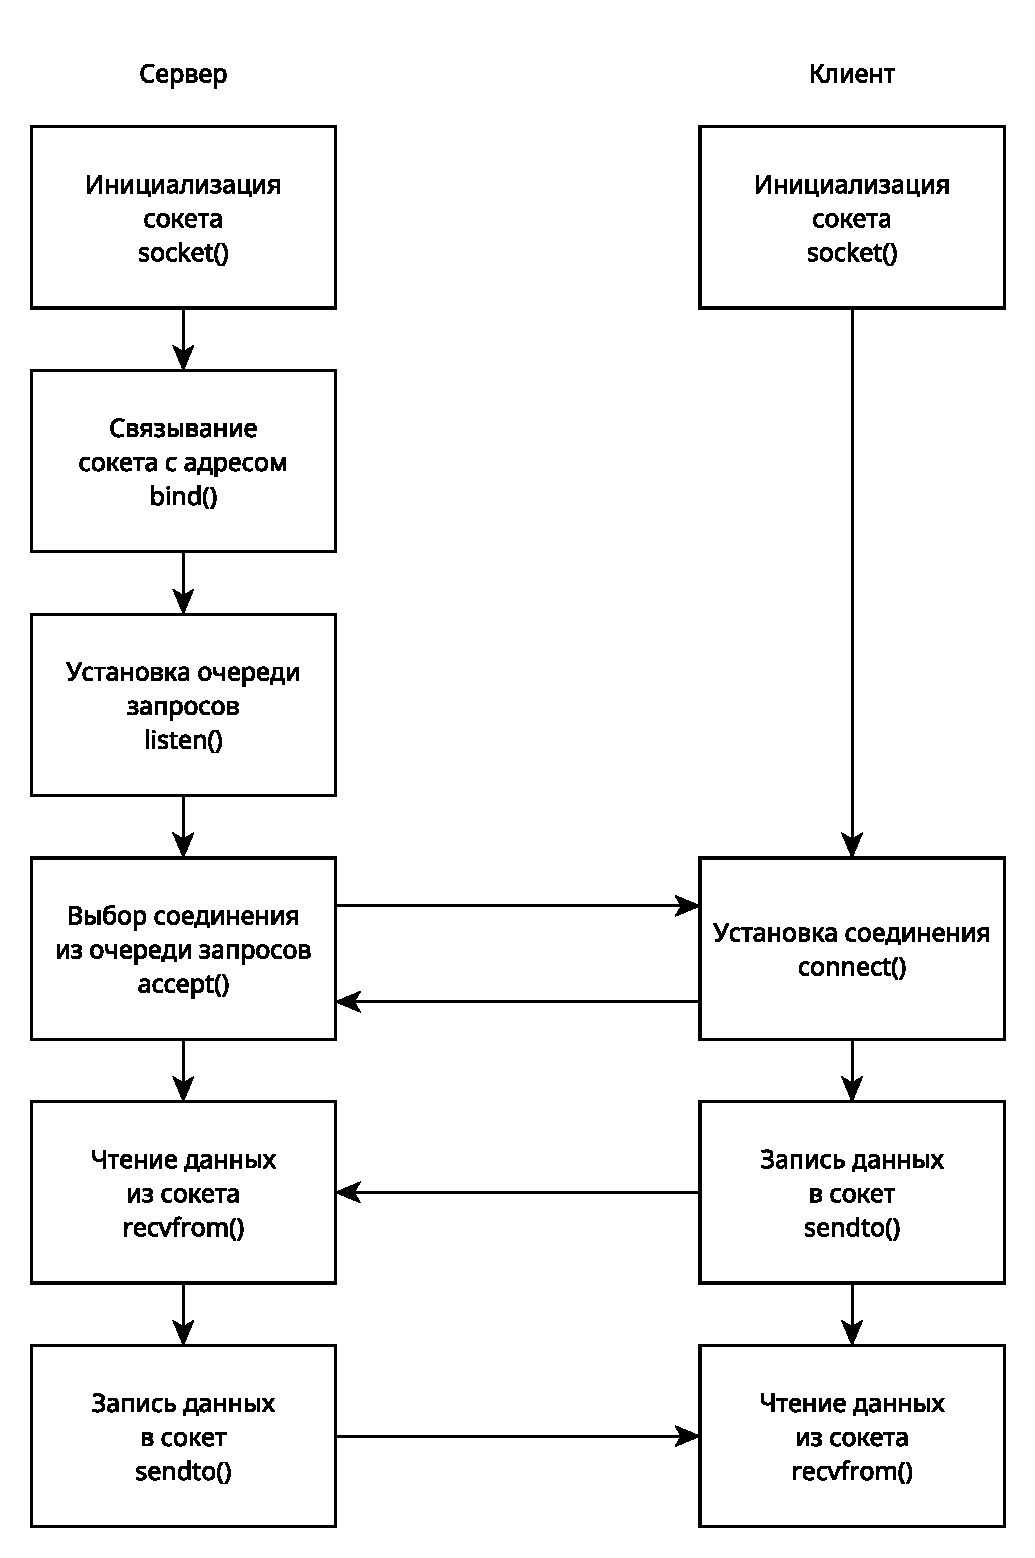
\includegraphics[width=0.9\linewidth]{linux_sock}
	\caption{Процесс установления соединения и обмена данными между сокетами сервера и клиента в операционной системе Linux}
	\label{linux_sock}
\end{figure}

\section{Разработка алгоритмов, необходимых для работы статического веб-сервера}

На рисунке~\ref{serv_alg} представлена схема алгоритма работы статического сервера.
\begin{figure}[H]
	\centering
	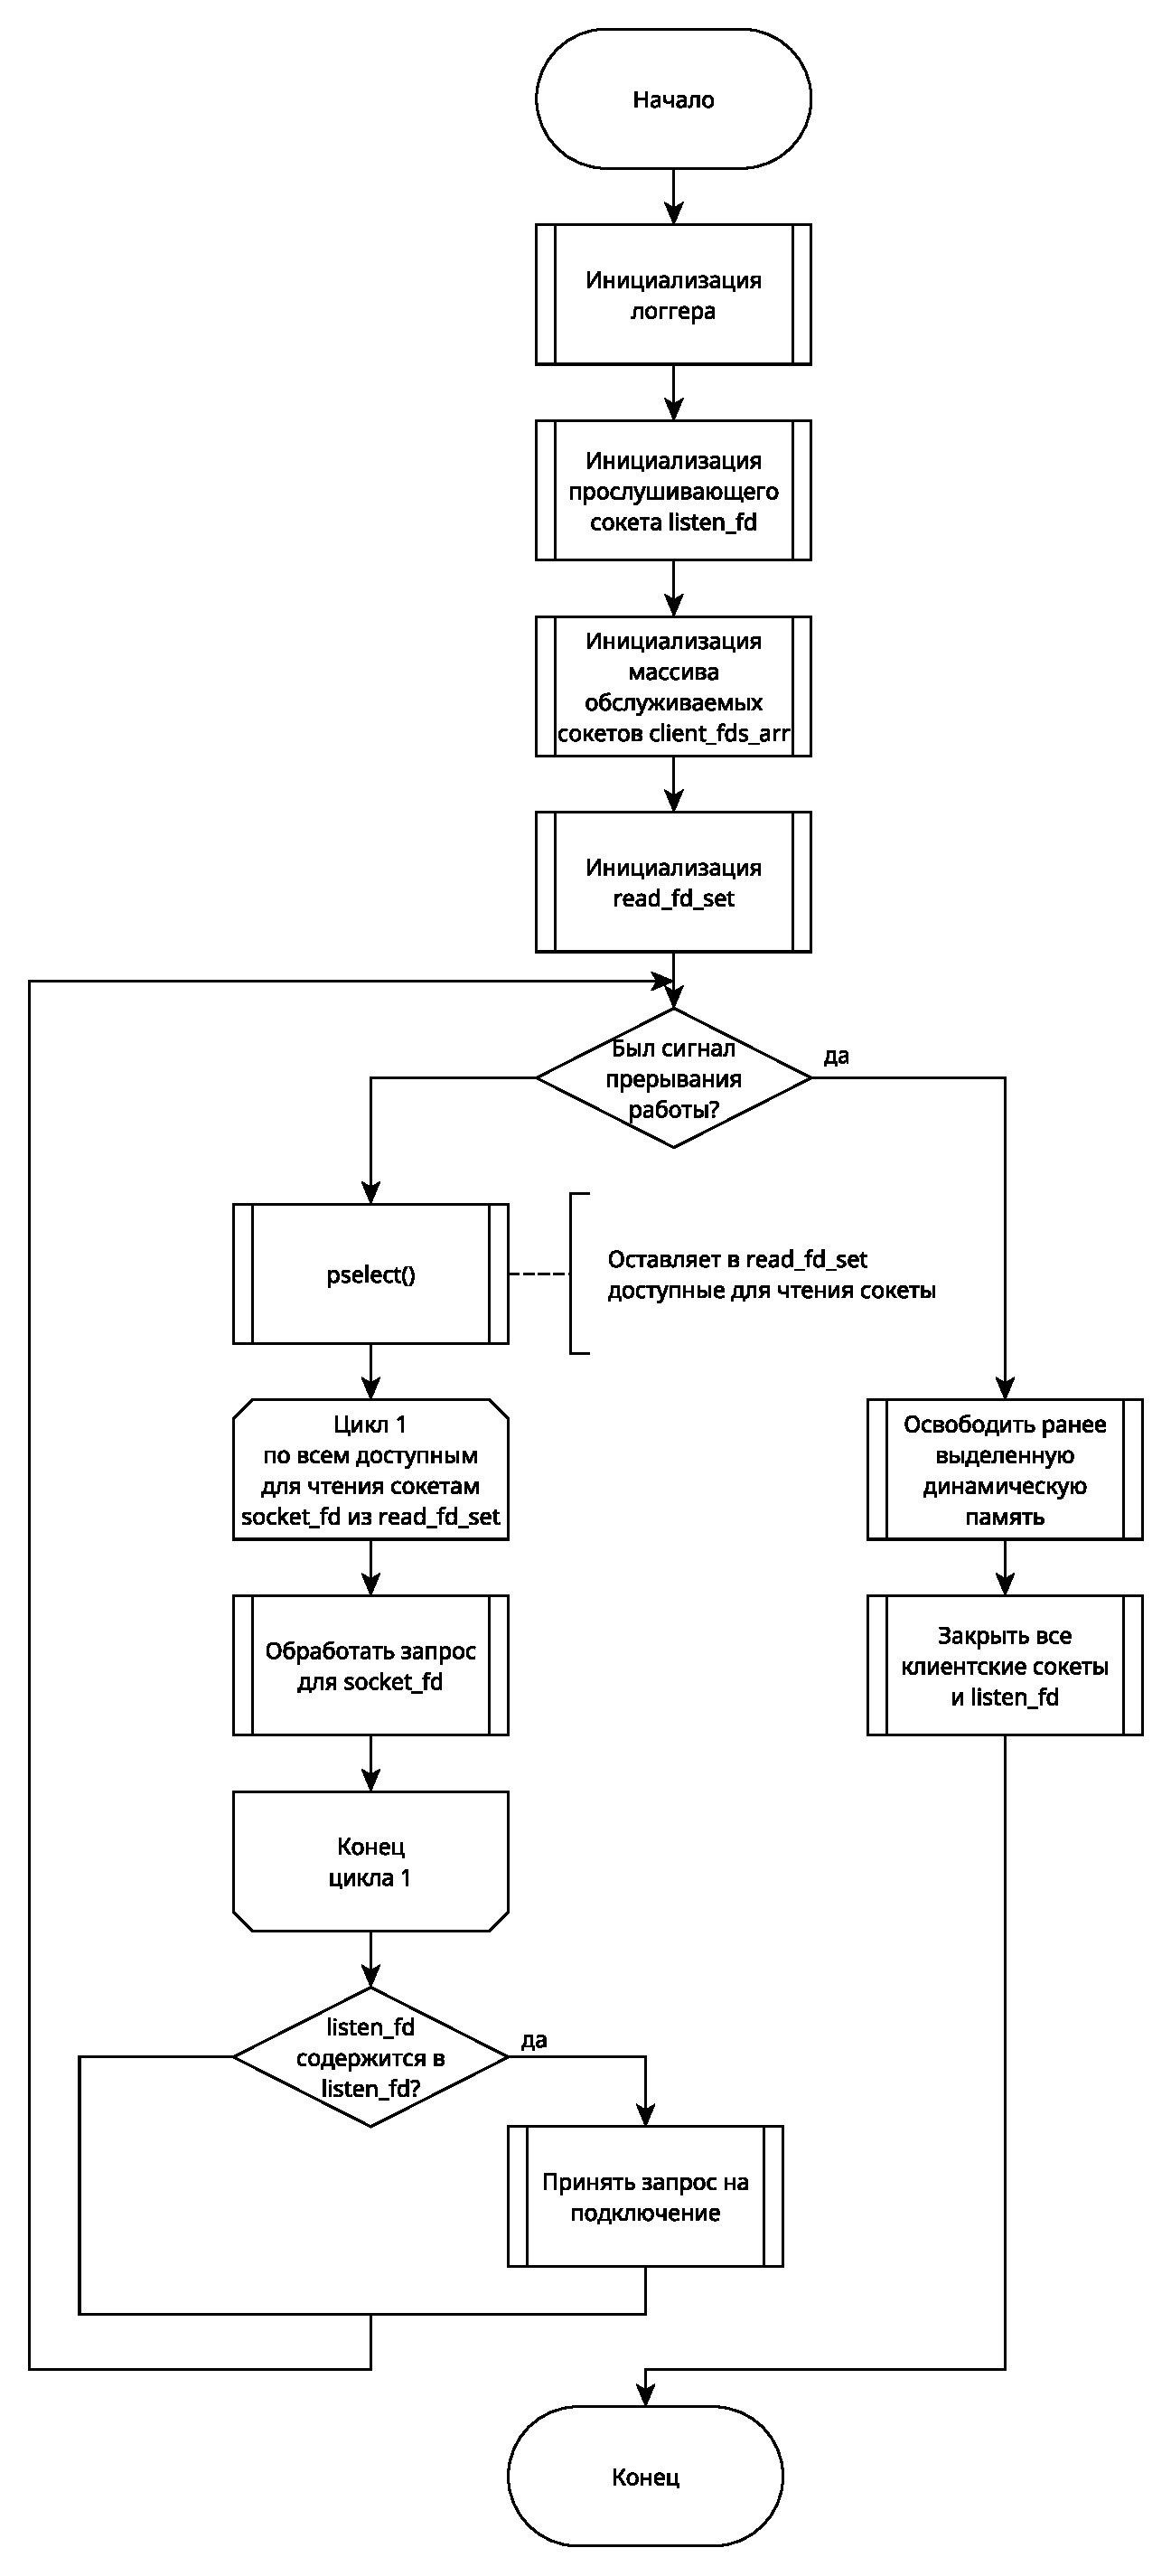
\includegraphics[width=0.58\linewidth]{serv_alg}
	\caption{Схема алгоритма работы статического сервера}
	\label{serv_alg}
\end{figure}

На рисунке~\ref{http_alg} представлена схема алгоритма обработки HTTP-запроса.
\begin{figure}[H]
	\centering
	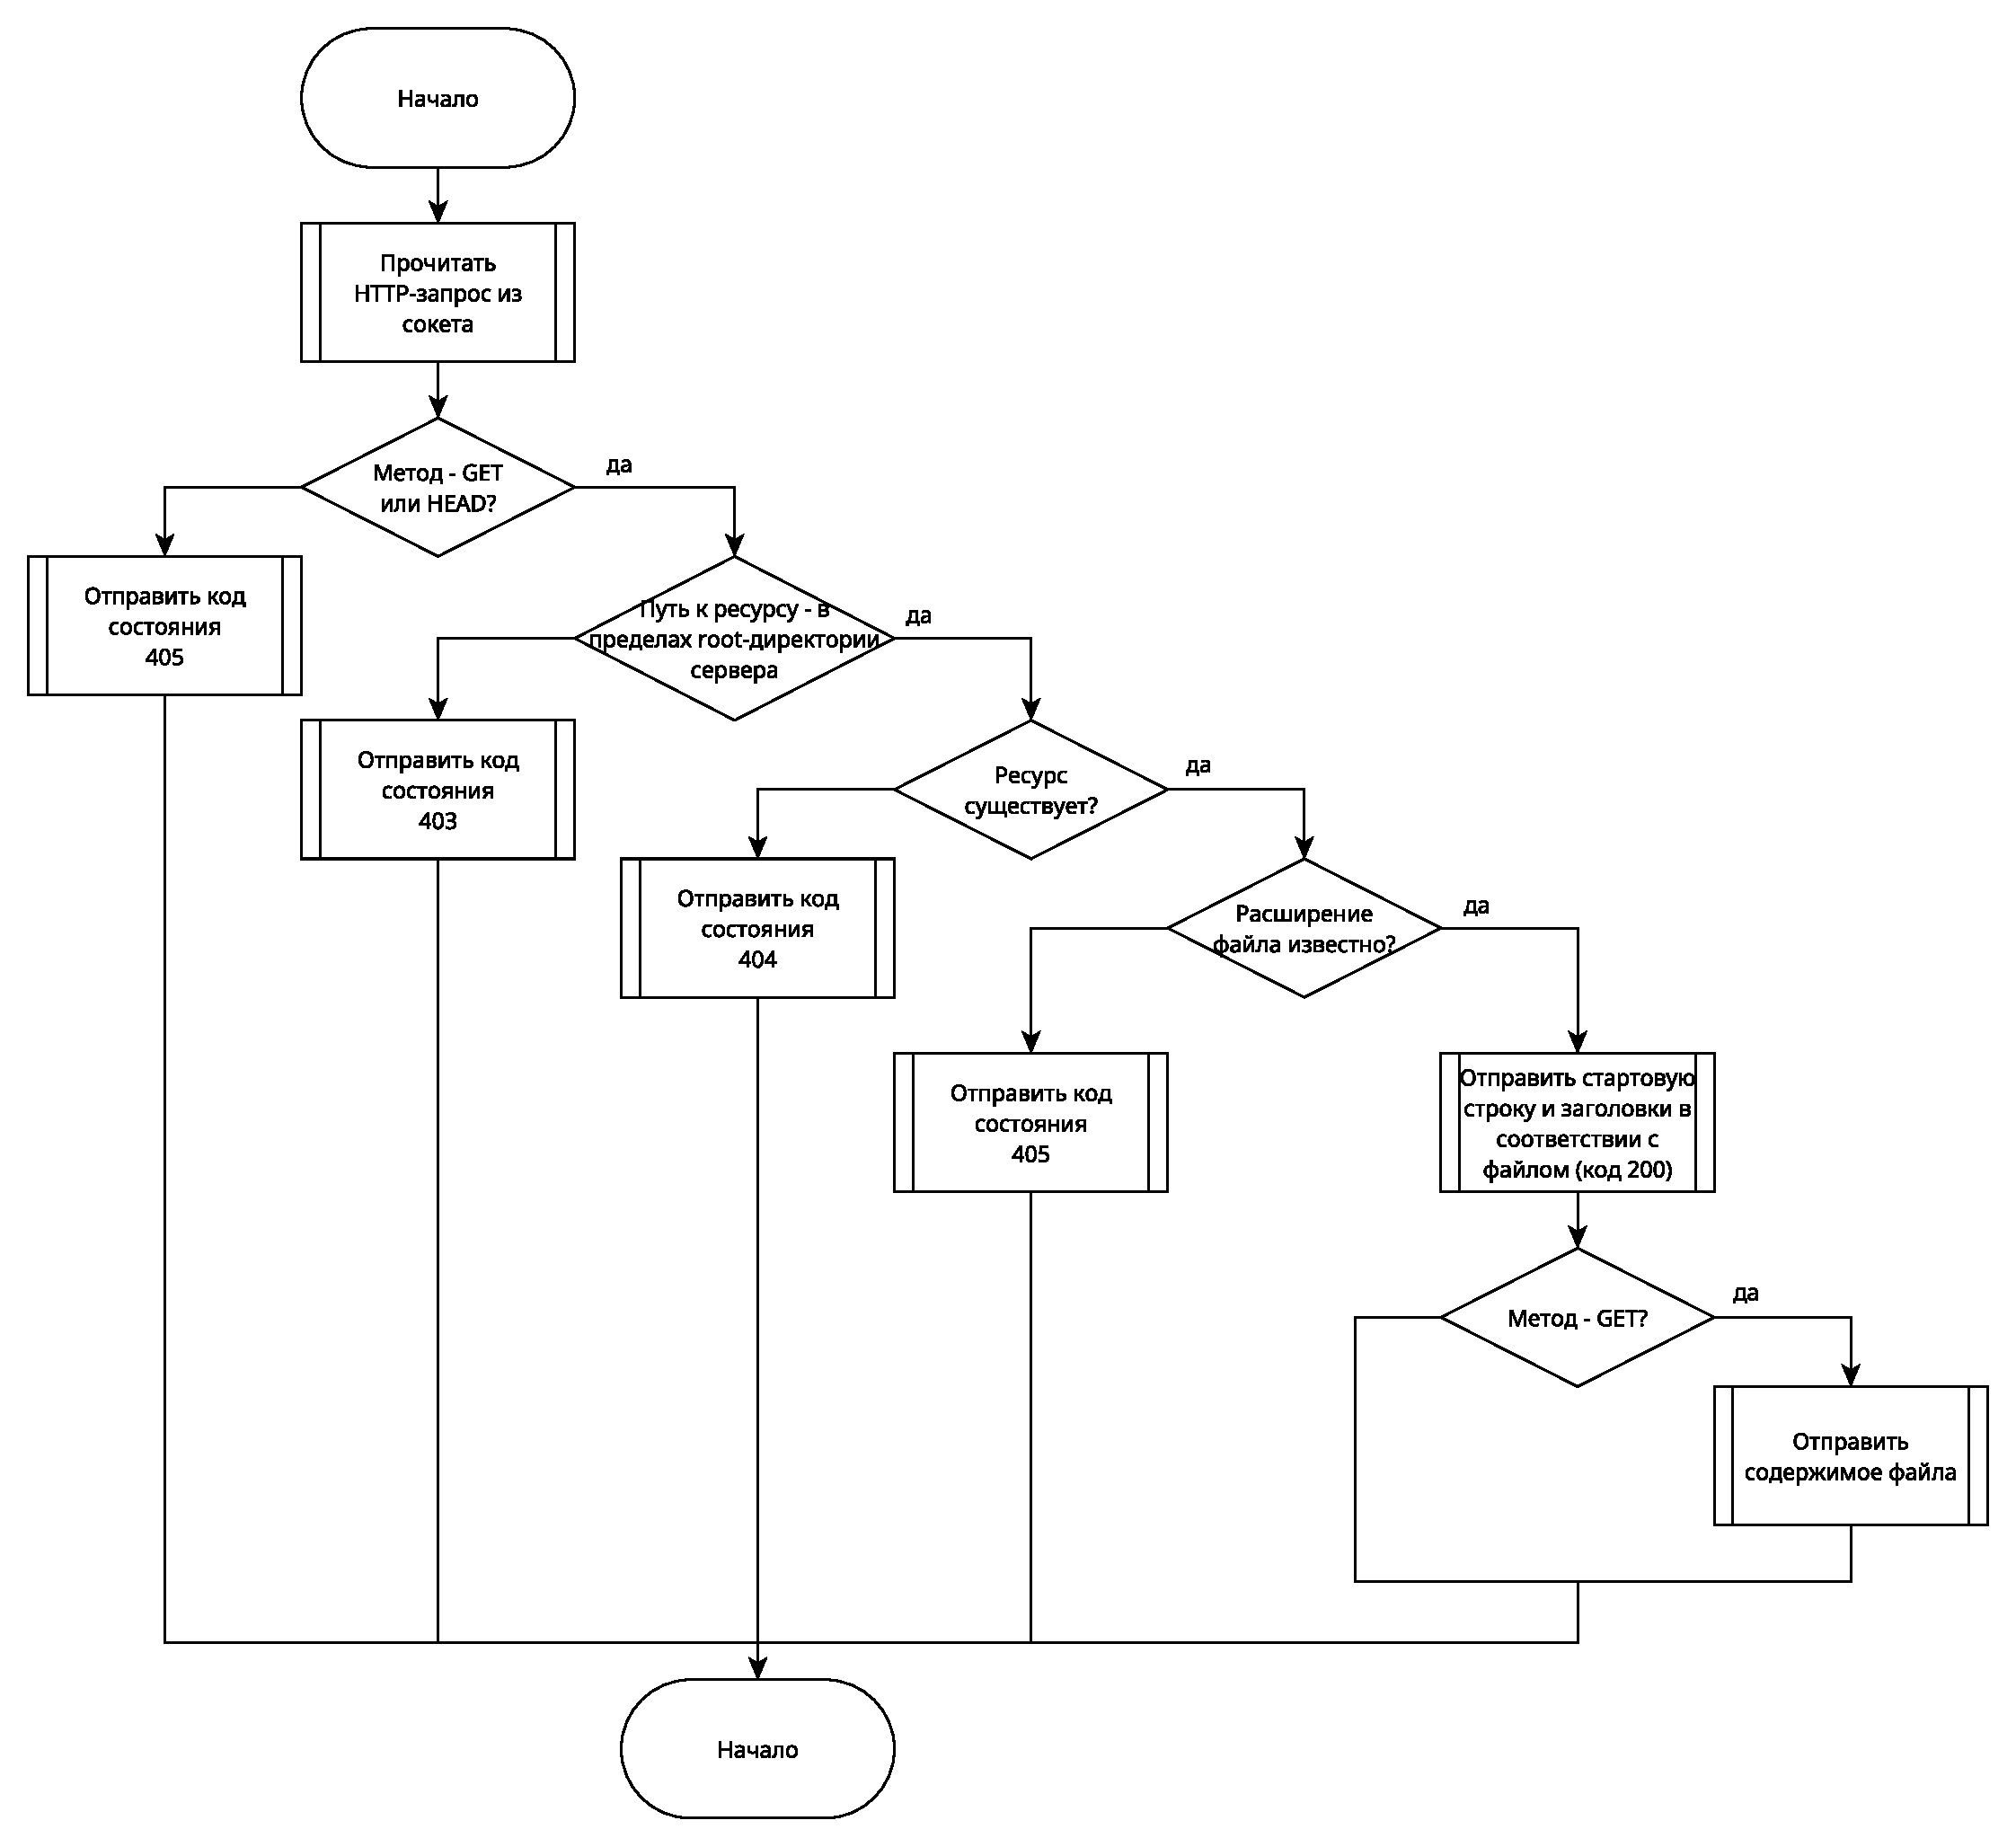
\includegraphics[width=\linewidth]{http_alg}
	\caption{Схема алгоритма обработки HTTP-запроса}
	\label{http_alg}
\end{figure}

\section*{Вывод}

Были сформулированы требования к разрабатываемому статическому веб-серверу.
Были проанализированы сокеты как средство взаимодействия между процессами.
Были разработаны схемы алгоритмов работы статического веб-сервера и обработки HTTP-запросов.

\clearpage
